\documentclass{article}
\usepackage{arxiv}

\usepackage[utf8]{inputenc} % allow utf-8 input
\usepackage[T1]{fontenc}    % use 8-bit T1 fonts
\usepackage{url}            % simple URL typesetting
\usepackage{booktabs}       % professional-quality tables
\usepackage{amsfonts}       % blackboard math symbols
\usepackage{amsmath}
\usepackage{nicefrac}       % compact symbols for 1/2, etc.
\usepackage{microtype}      % microtypography
\usepackage{lipsum}
\usepackage{caption}
\usepackage{graphicx}
\usepackage{minted} 
\usepackage{hyperref}       % hyperlinks

\usepackage{xcolor}
\definecolor{bg}{rgb}{0.95, 0.95, 0.92}

\title{News broadcast analysis}


\author{
	Christine K. C. Cheng
}

\begin{document}
\maketitle

\section{Shot detection}
\subsection*{Sum of absolute differences}
A score is assigned to each frame by calculating the sum of the absolute differences between consecutive frames for every pixel. This value is then normalized by the size of the frame. A threshold is selected through empirical experiments before score calculations. When the score of a frame is greater than the threshold, a shot change is declared.
This method works quite well with simple videos but it is not robust against movements and changes in lighting.

\subsection*{Histogram differences}
Each frame is converted into a gray-scale image. A histogram with 256 bins, representing all the possible values of a pixel, is created for each frame. Then, a score is assigned by calculating the sum of the absolute differences between histograms of consecutive frames.

\begin{minipage}{0.5\linewidth}
\captionof{figure}{Sum of absolute differences scores of clip 1} \label{fig: clip_1_sad2}
\centering
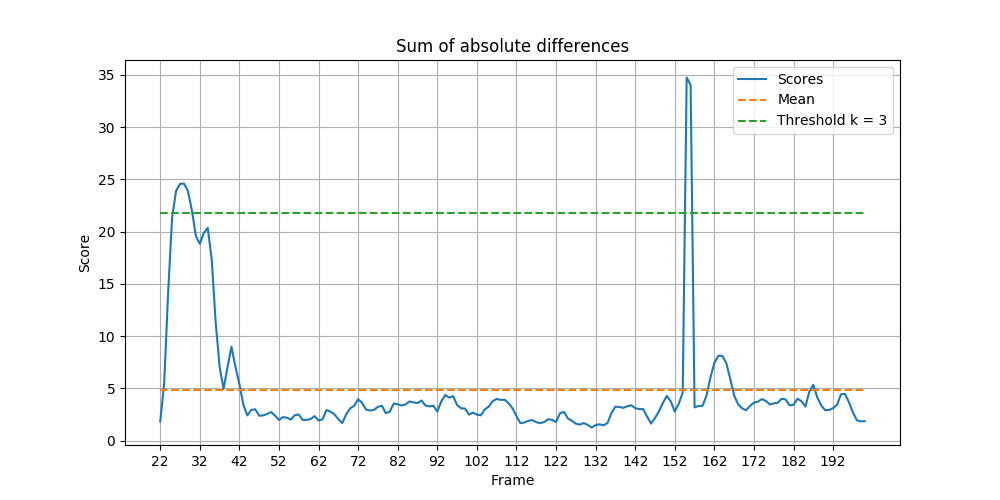
\includegraphics[width=3.5in]{../output/clip_1_score_sad2.png}
\end{minipage}%
\begin{minipage}{0.5\linewidth}
\captionof{figure}{Histogram differences scores of clip 1} \label{fig: clip_1_hd}
\centering
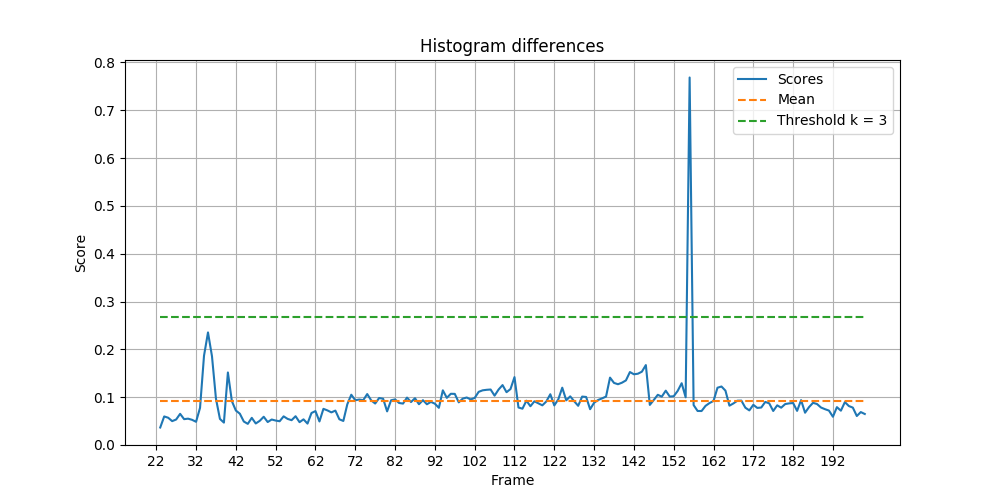
\includegraphics[width=3.5in]{../output/clip_1_score_hd.png}
\end{minipage}

\begin{minipage}{0.5\linewidth}
\captionof{figure}{Sum of absolute differences scores of clip 2} \label{fig: clip_2_sad2}
\centering
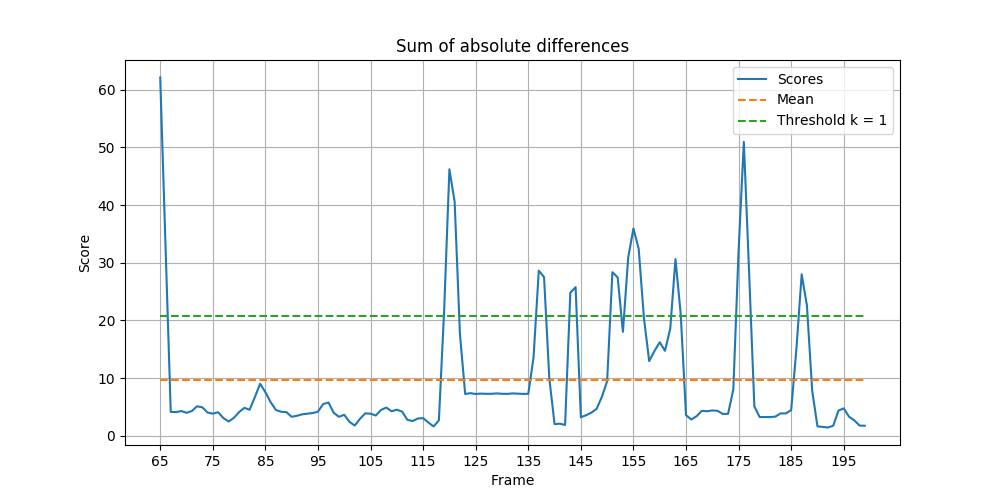
\includegraphics[width=3.5in]{../output/clip_2_score_sad2.png}
\end{minipage}%
\begin{minipage}{0.5\linewidth}
\captionof{figure}{Histogram differences scores of clip 2} \label{fig: clip_2_hd}
\centering
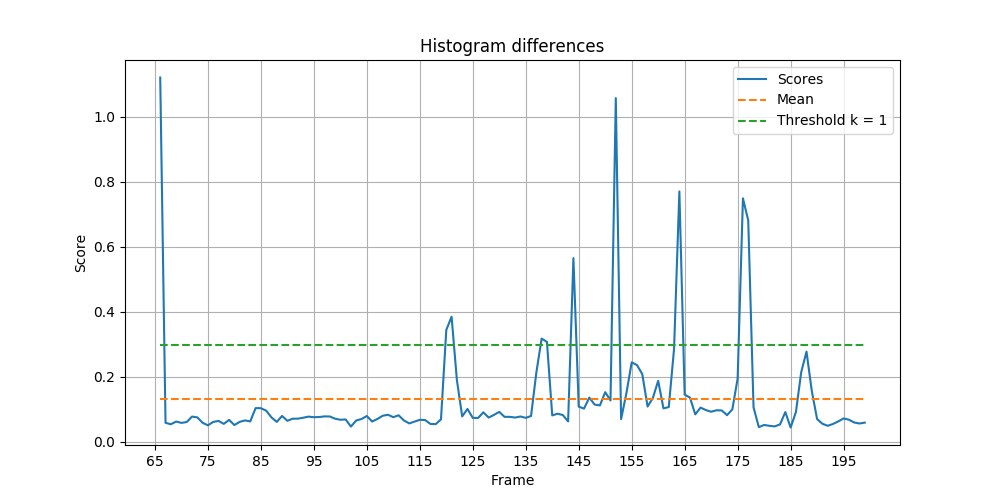
\includegraphics[width=3.5in]{../output/clip_2_score_hd.png}
\end{minipage}

\begin{minipage}{0.5\linewidth}
\captionof{figure}{Sum of absolute differences scores of clip 3} \label{fig: clip_3_sad2}
\centering
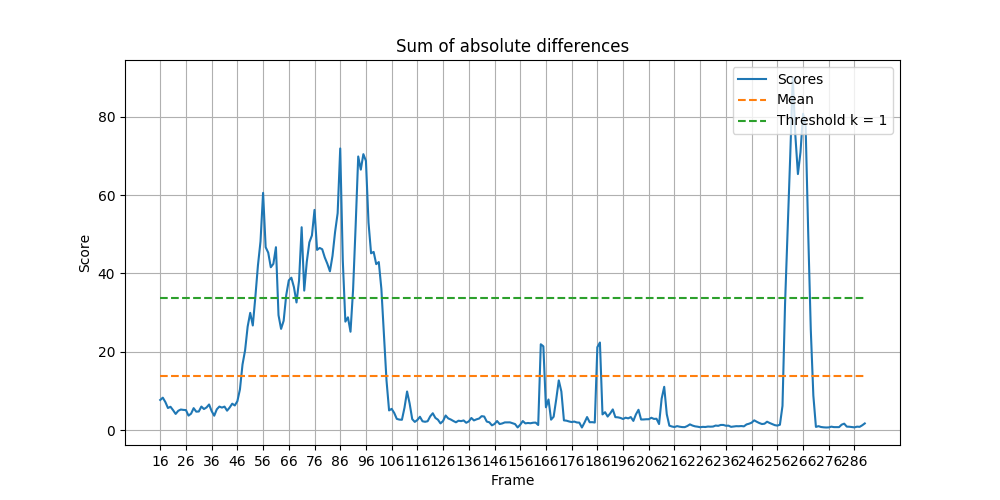
\includegraphics[width=3.5in]{../output/clip_3_score_sad2.png}
\end{minipage}%
\begin{minipage}{0.5\linewidth}
\captionof{figure}{Histogram differences scores of clip 3} \label{fig: clip_3_hd}
\centering
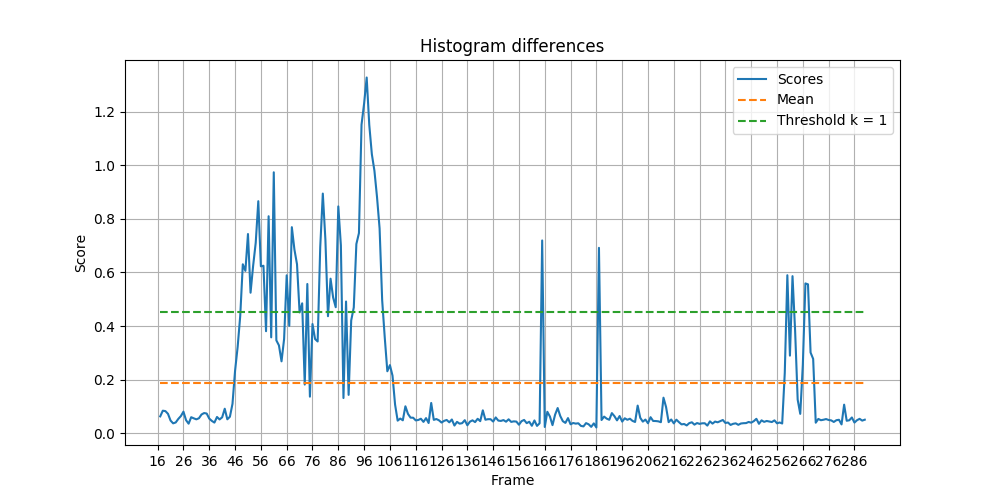
\includegraphics[width=3.5in]{../output/clip_3_score_hd.png}
\end{minipage}

The relevant code is in \texttt{shot.py}. To get the graphs of shot detection, run the command below. 
\begin{minted}[bgcolor=bg]{sh}
python3 run.py shot_detection -t <type> -i <path to frames>
\end{minted}

\section{Logo detection}
Template matching is an object detection algorithm which is translation invariant but not scale or rotation invariant. As we are detecting a logo, it is assumed that the target of detection will be in a known orientation. Also, template matching is run on templates of different sizes because the size of the logo in a frame is unknown. 

Due to the possibility that there may be multiple occurrences of the logo in a frame, we cannot simply match SIFT features between the logo and a frame. 

\begin{minipage}{\linewidth}
\captionof{figure}{Logo detection on clip 1} \label{fig: logo}
\centering
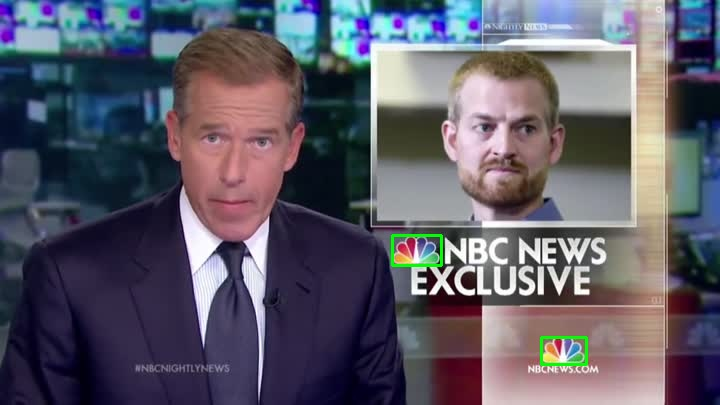
\includegraphics[width=2.5in]{../output/clip_1_logo/052.jpg}
\end{minipage}

The relevant code is in \texttt{logo.py}. To run logo detection, run the command below.
\begin{minted}[bgcolor=bg]{sh}
python3 run.py logo_detection -i <input directory> -o <output directory>
-d <logo path> -t <min threshold>
\end{minted}

\section{Face detection}
There are 260 images in the female and male classes respectively. Each image is accompanied by a \texttt{.mat} file specifying the coordinates of the left eye, right eye, nose and mouth. The following rules are used to crop the images in order to obtain the faces.
\begin{equation}
\begin{split}
start_x &= left~eye_x - 0.5\times(right~eye_x - left~eye_x) \\
end_x &= right~eye_x + 0.5\times(right~eye_x - left~eye_x) \\
start_y &= eyes_y - (mouth_y - eyes_y) \\
end_y &= mouth_y + (mouth_y - eyes_y) \\
\end{split}
\end{equation}

\subsection*{Color detection}
The initial attempt to detect faces is to use skin detection - trying to filter out skin in images. Figure \ref{fig: rgb} and Figure \ref{fig: hsv} show the color distributions of faces in RGB and HSV color spaces. The HSV color space has narrower distributions, especially with hue. Although this method works sometimes as seen in Figure \ref{fig: hsv_good}, it is not successful in general. It fails to detect a large area of the face of the man on the right in Figure \ref{fig: hsv_bad}. Also, this model is especially poor when other things in the frame are very similar to human skin tone.

\begin{minipage}{0.5\linewidth}
\captionof{figure}{RGB distribution of fe male training images} \label{fig: rgb}
\centering
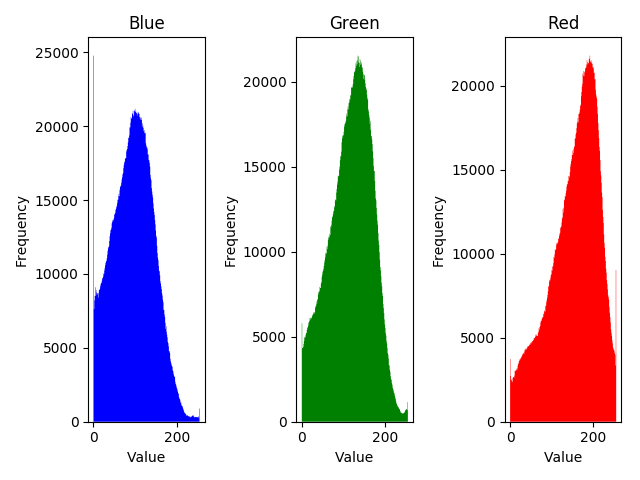
\includegraphics[width=2.5in]{../output/f_train_rgb_distributions.png}
\end{minipage}%
\begin{minipage}{0.5\linewidth}
\captionof{figure}{HSV distribution of female training images} \label{fig: hsv}
\centering
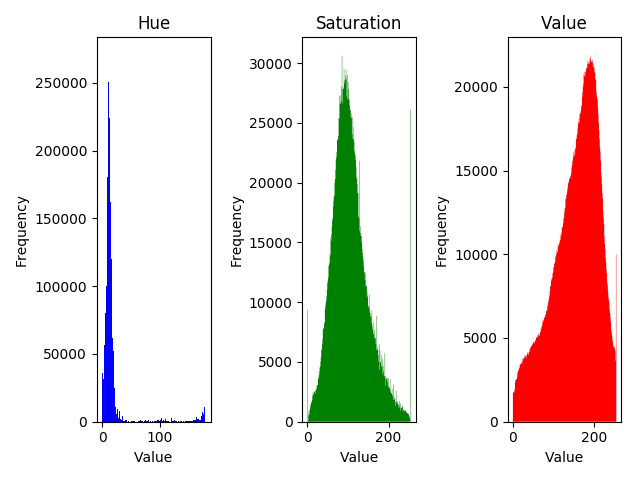
\includegraphics[width=2.5in]{../output/f_train_hsv_distributions.png}
\end{minipage}

\begin{minipage}{0.5\linewidth}
\captionof{figure}{HSV distribution of female training images} \label{fig: hsv_good}
\centering
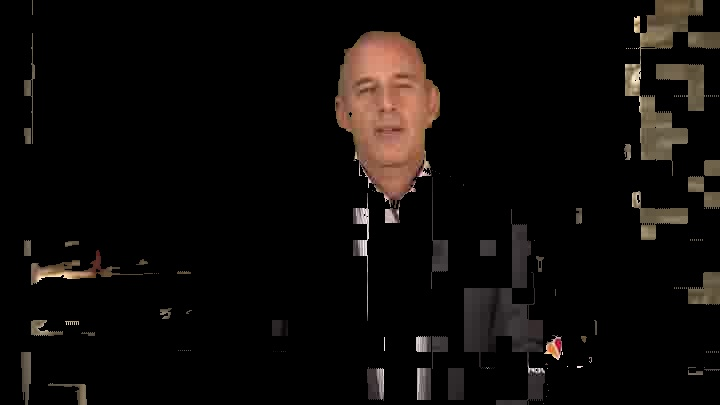
\includegraphics[width=2.5in]{../output/clip_1_hsv/160.jpg}
\end{minipage}
\begin{minipage}{0.5\linewidth}
\captionof{figure}{HSV distribution of female training images} \label{fig: hsv_bad}
\centering
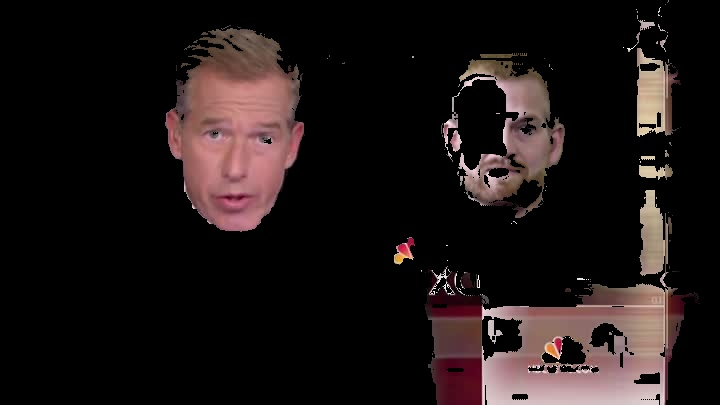
\includegraphics[width=2.5in]{../output/clip_1_hsv/050.jpg}
\end{minipage}

\subsection*{Classifier}
I ended up using \texttt{cv2.CascadeClassifier} for detecting faces. It works fairly well. However, it was not able to detect the face in Figure ????? despite trying different parameters.

\section{Gender classification}
90\% of the images were used for training, whereas the other 10\% were used for testing the accuracy of the model.

\subsection*{SVM}
The SIFT descriptors of the training images are passed into the SVM model for training.
For each detected face, the SIFT descriptors are extracted and fed to the trained SVM model. Then, a prediction for each descriptor is obtained. If more descriptors are predicted as female than male, the image is classified as female. If more descriptors are predicted as male than female, the image is classified as male. If there are equal number of descriptors being predicted as both female and male, the image is then classified as unknown.

\subsection*{Neural network}
The same as SVM, except with a neural network model instead. The model uses a binary crossentropy loss, adam for optimization, and accuracy as the metric. 

\subsection*{CNN}
All the training and testing images are padded with black borders to obtain a square shape and then resized to be 72 pixels by 72 pixels. The training images are then passed to the CNN model shown in Figure \ref{fig: cnn_model} for training. The model uses a binary crossentropy loss, stochastic gradient descent for optimization, and accuracy as the metric.
Each detected face is padded to obtain a square shape. Then, the image is resized to be 72 pixels by 72 pixels. The resized image is then passed to the trained cnn model and a category prediction is obtained.

\begin{minipage}{\linewidth}
\captionof{figure}{CNN model} \label{fig: cnn_model}
\centering
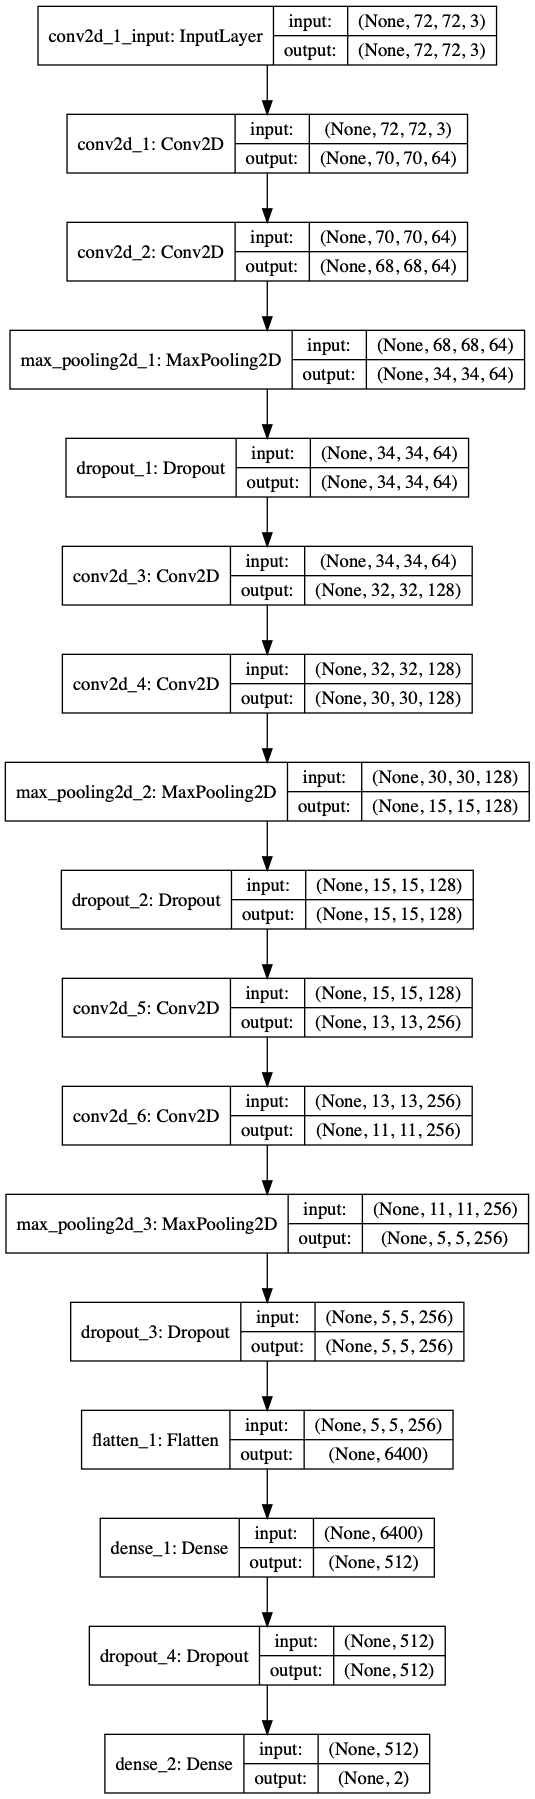
\includegraphics[width=2.5in]{../output/cnn_model.png}
\end{minipage}

The relevant code is in \texttt{train\_model()} in \texttt{face.py}. To train a gender classification model, run the command below.
\begin{minted}[bgcolor=bg]{sh}
python3 run.py train -m <model path after training> 
-c <classification model (SVM, NN_SIFT, or CNN)>
\end{minted}

The relevant code for face detection (including gender classification) is in \texttt{face\_detection()} in \texttt{face.py}. Run the command below.
\begin{minted}[bgcolor=bg]{sh}
python3 run.py face_detection -i <input directory> -o <output directory>
-c <classification model (SVM, NN_SIFT, or CNN)> -m <trained model path> 
\end{minted}

\subsection*{Performance}
Table \ref{tab:gender_classification} shows the test accuracies of the three models. As expected, CNN performed poorly, as good as random guesses, due to the very small training data size of 468.

\begin{table}[h]
 \caption{Gender classification performance}
  \centering
  \begin{tabular}{lll}
    \toprule
    Model		& Description														& Accuracy on test set \\
    \midrule
    SVM							& 	Using SIFT descriptors of faces						& 100.00\% \\
    Neural network		& Using SIFT descriptors of faces							& 92.30\% \\
    CNN							&	Using cropped and resized faces						& 50.00\% \\
    \bottomrule
  \end{tabular}
  \label{tab:gender_classification}
\end{table}

\section{References}
\href{https://www-nlpir.nist.gov/projects/tvpubs/tvpapers03/ramonlull.paper.pdf}{Video shot boundary detection based on color histogram}

\href{https://en.wikipedia.org/wiki/Shot_transition_detection}{Wikipedia - Shot transition detection}

\end{document}